\section*{Introduction} 
% To give the unnumbered section a line in the table of contents:
\addcontentsline{toc}{section}{Introduction} 
% To add the correct header text for this section:
% (Otherwise it says CONTENTS from the previous section.)
\markright{INTRODUCTION}

The following example is intended to illustrate how calculus is applied in other fields.  You don't have to follow every step at this stage (although some of you will).  By the end of the unit, you should be able to tackle more complex examples.

\begin{example}

Application: predicting global population.

Population is a function $u(t)$ of time $t$.

Express this as:
 \begin{description}
\item[A.] \textbf{Table}

\begin{center}
\begin{tabular}{| c | c |}
\hline
Year & Population (millions)\\
\hline
1000 & 310 \\
\hline 1800 & 978 \\
\hline 1900 & 1650 \\
\hline 1990 & 5263 \\
\hline 2000 & 6070 \\
\hline 2008 & 6707\\
\hline 2008 & 6707 \\
\hline 2010 & 6873 \\
\hline
\end{tabular}
\end{center}


\item[B.] \textbf{Graph} (figure (\ref{expgrowth}))

%\nextalt{Axes $u$ against $t$. Sketch of a curve showing exponential growth.}
\begin{figure}[!hbtp]
\centering
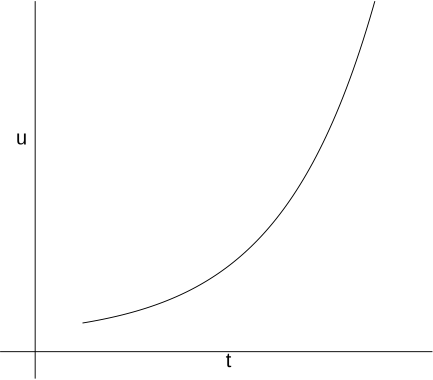
\includegraphics[width=0.5\textwidth]{exp_growth.pdf}
\caption{Exponential growth}
\label{expgrowth}
\end{figure}

\newpage

\item[C.] \textbf{Differential equation}


Population is $u(t)$. What is the \textbf{rate of change} of the
population?

In a time interval $\delta t$:
\begin{itemize}
\item A proportion $a \delta t$ of population produce
children.

\item A proportion $b \delta t$ of population die.

\item A proportion $c \delta t$ of population emigrate to Mars.
\end{itemize}

So,
\begin{align*}
& u(t + \delta t)  =  u(t) + (a-b-c)u(t) \delta t  \\
\Longrightarrow & \dfrac{u(t+\delta t) - u(t)}{\delta t} =
\lambda u(t),
\end{align*}
where $\lambda = a - b - c$.

\end{description}

Let $\delta t \to 0$ (see analysis course).

Then
  \begin{align*}
    \dfrac{du(t)}{dt} & =  \lambda u(t)  \\
    u(t_{0}) & = u_{0}
  \end{align*}

A differential equation like this, describing population growth, was used by Thomas Malthus, early 19th century.

\subsection*{Parameter estimation}

The UN estimates that the population grows by $1.14\%$ per year.

Let $t$ be time in years.

We separate the variables in our differential equation, then integrate (details later, when we study differential equations).
  \begin{align*}
    \dfrac{du}{dt} & = \lambda u  \\
    \implies \int \dfrac{1}{u} \, du & = \int \lambda \, dt  \\
    \implies u(t) & = u_{0} e^{\lambda(t-t_{0})}
  \end{align*}

We are interested in the change over one year, so let $t_{0}=t$, so $u_{0}=u(t)$, and consider
  \begin{align*}
    u(t + 1) & = u(t)e^{\lambda(t + 1 - t)}  \\
    & = u(t)e^{\lambda}  \\
    \implies \frac{u(t+1)-u(t)}{u(t)} & = \frac{u(t)e^{\lambda} - u(t)}{u(t)}  \\
    & = e^{\lambda} - 1.
  \end{align*}
This is the proportional increase in population over one year, so the UN estimate tells us that
  \begin{align*}
    e^{\lambda} - 1 & = 0.0114 \qquad (1.14\% \text{ growth})  \\
    \implies \lambda & = \ln (1+ 0.0114) \approx 0.01133551
  \end{align*}

Hence
\[
 u(t) = u_{0} e^{0.01133551(t-t_{0})}
\]
\end{example}

\subsection*{Application}

How long would it take for the population to double?

Pros:
\begin{itemize}[topsep=0pt]
\item Model easy to solve
\item Gives testable predictions
\end{itemize}

Cons:
\begin{itemize}[topsep=0pt]
 \item Unrealistic -- does not include effects of resource depletion, over-crowding, medical advances, agricultural advances, etc.
\end{itemize}

% I've cut this next paragraph because (a) I didn't like it; (b) the third point is vague/meaningless; (c) the fourth point makes the whole thing self-defeating (as, indeed, this kind of maths is).
%Generally
%\begin{itemize}[topsep=0pt]
% \item Use of differential equations started with Newton.
% \item Differential equations arise in many fields, including the sciences, engineering, economics, astronomy, etc.
% \item Very powerful approach.
% \item Most realistic models need a computer to solve.
%\end{itemize}

% This bit now unfortunately spills onto another page.
% (This sort of thing probably goes to pot when typesetting in large print anyway.)
To construct more realistic models, we will need to be able to
  \begin{itemize}[topsep=0pt]
    \item work with more than one independent variable;
    \item construct and solve more complex differential equations;
    \item evaluate more complex integrals.
  \end{itemize}


